\documentclass[
  lualatex,
  aspectratio=169,
  14pt
]{beamer}

\usetheme[progressbar=frametitle]{Metropolis}
%\setbeameroption{show notes on second screen=bottom}

\usepackage{xparse}
\usepackage{mathtools,amssymb}
\usepackage{graphicx,xcolor}
\usepackage{pxrubrica}
\usepackage{calc}
\usepackage[absolute,overlay]{textpos}
\usepackage{enumitem}
\usepackage[1.7]{bxpdfver}
\usepackage{pdfcomment}
\usepackage{ulem}
\usepackage{stackengine}
\usepackage{appendixnumberbeamer}

% フォント
\usepackage[lining,tabular,sfdefault]{FiraSans}
\usepackage[mathrm=sym,mathbf=sym]{unicode-math}
\setmathfont{Fira Math}
\usepackage[no-math,deluxe,haranoaji]{luatexja-preset}
\RenewDocumentCommand\kanjifamilydefault{}{\gtdefault}

% 打ち消し線関連
\RenewDocumentCommand\ULthickness{}{.1\zh}
% 二重打ち消し
\NewDocumentCommand\dsout{m}{%
  \stackengine{.2\zh}{#1}{%
    \stackengine{-.3\zh}{\sout{\hphantom{#1}}}{\sout{\hphantom{#1}}}{O}{c}{F}{F}{L}%
  }{O}{c}{F}{F}{L}}

% 下に文字置くやつ
\NewDocumentCommand\replace{mm}{%
  \stackengine{-1\zh}{\dsout{#1}}{#2}{O}{c}{F}{F}{L}}

\usepackage{hyperref}

\title{オレオレIP電話網を大きくしたら\\
Tailscaleの\texorpdfstring{\replace{不具合}{ワナ}}{ワナ}を踏み抜いて発狂した話}
\subject{エンジニア作業飲み集会\#125}
\author{上羽 未栞(a.k.a. KusaReMKN)}
\institute{%
  \href{https://tkytel.github.io/}{東京広域電話網〈\url{https://tkytel.github.io/}〉}\\
  \url{https://KusaReMKN.com/}\\
  Twitter: \href{https://twitter.com/KusaReMKN}{@KusaReMKN}}
\keywords{Tailscale; 黒電話; VoIP; IP電話; MikoPBX; 東京広域電話網}
\date{2025-05-16}

\begin{document}

\begin{frame}
  \titlepage
  \note{
    発表を始めるよ。
    「オレオレIP電話網を大きくしたらTailscaleのワナを踏み抜いて発狂した話」と題して、
    みかんちゃんが発表するよ。
  }
\end{frame}

\begin{frame}
  \frametitle{今回のおはなし}

  ~\\[-.25\baselineskip]
  \tableofcontents
  \note{
    今回の発表の流れはこんな感じだよ。
    質疑応答を含めて大体20分間くらいで進められたらいいな。
  }
\end{frame}

\section*{みかんちゃんについて}
\note{
  自己紹介するよ。
}

\begin{frame}
  \frametitle{自称・大天才美少女プログラミング初心者}

  \begin{textblock*}{0.5\paperwidth}(0.6cm, 3.5cm)
    
\includegraphics[width=0.3\paperwidth]{./images/mikanchan.png}
  \end{textblock*}
  \begin{columns}
    \begin{column}{0.30\textwidth}
      \\~\\[-.25\baselineskip]
    \end{column}
    \begin{column}{0.69\textwidth}
      \\~\\[-.25\baselineskip]
      「\ruby{上羽}{うわ|ば} \ruby{未栞}{み|かん}」
      あるいは「\ruby[g]{KusaReMKN}{くされみかん}」\\
      \hspace{1.5\zw}\textbf{みかんちゃん}って呼んでね!
      \\~\\[-.5\baselineskip]

      実はプログラマでもエンジニアでもない\\
      \hspace{1.5\zw}古い計算機っぽいものが大好き\\
      \hspace{1.5\zw}最近は電話機などにも目がない
      \\~\\[-.5\baselineskip]

      Twitterで思想を垂れ流すことが得意\\
      \hspace{1.5\zw}\url{https://kusaremkn.com/}も見てね
    \end{column}
  \end{columns}
  \note{
    大天才美少女プログラミング初心者を自称している、上羽未栞だよ。
    みかんちゃんって呼ばれると大変喜ぶよ。

    大天才とかプログラミング初心者とか言っているけれど、
    実はプログラマでもエンジニアでもないよ。
    外の人(学生のすがた)は通信方式について研究していたりするけれど、
    それはまた別のお話だよ。
    それはそれとして古い計算機っぽいものが大好きだよ。
    よくハードオフに出没してジャンク箱を小豆洗いしているよ。
    最近は電話機などにもお熱で、家に電話機が20台以上発生していて困っているよ。

    Twitterとかウェブサイトとかあるよ。
    暇な人は覗いてみてね。
    深淵があるよ。
  }
\end{frame}

\section{東京広域電話網について}
\note{
  みかんちゃんたちがやっているオレオレIP電話網「東京広域電話網」について説明するよ。
}

\begin{frame}
  \frametitle{分散型の異常オレオレIP電話網}

  \textbf{東京広域電話網}
  (\textit{Tokyo Wide Area Telephony Network})\\
  \hspace{1.5\zw}Telephone for Everyone, Connecting Heritages
  \\~\\[-.5\baselineskip]

  2024年10月頃に発足したオレオレIP電話網\\
  \hspace{1.5\zw}VoIPサーバを設置して相互接続・電話網を構築\\
  \hspace{1.5\zw}黒電話やワープロなど異常な端末が数多く生息中
  \\~\\[-.5\baselineskip]

  2月21日のエンジニア作業飲み集会でLT発表\\
  \hspace{1.5\zw}電話局の数: 13 → 32\\
  \hspace{2.5\zw}端末の数: 58 → 198
  \hspace{1.5\zw}(2025-05-11現在)

  \note{
    東京広域電話網は分散型のオレオレIP電話網だよ。
    Telephone for Everyone, Connecting Heritagesをスローガンに、
    故き良き通信を楽しんでいるよ。

    東京広域電話網のプロジェクトは去年の10月に始まって、
    各人が各々の電話サーバを立てて相互に接続することで電話網を形成しているよ。
    黒電話やワープロなどの異常な端末が数多く生息しているよ。

    2月にエンジニア作業飲み集会でLTをしたときに大反響があって、
    それ以来網がだい成長しているよ(だいたい、全ての数字が倍になったよ)。
  }
\end{frame}

\begin{frame}
  \frametitle{現在の東京広域電話網の姿}

  \begin{columns}
    \begin{column}{.28\textwidth}
      \begin{description}[labelwidth=\linewidth]
        \item[交換局数]
          32局
        \item[端末数]
          198以上\\
          (仮想含む)
        \item[うち黒電話]
          22程度
        \item[その他]
          ピンク電話\\
          ISDNやPHS
      \end{description}
    \end{column}
    \begin{column}{.7\textwidth}
      \centering
      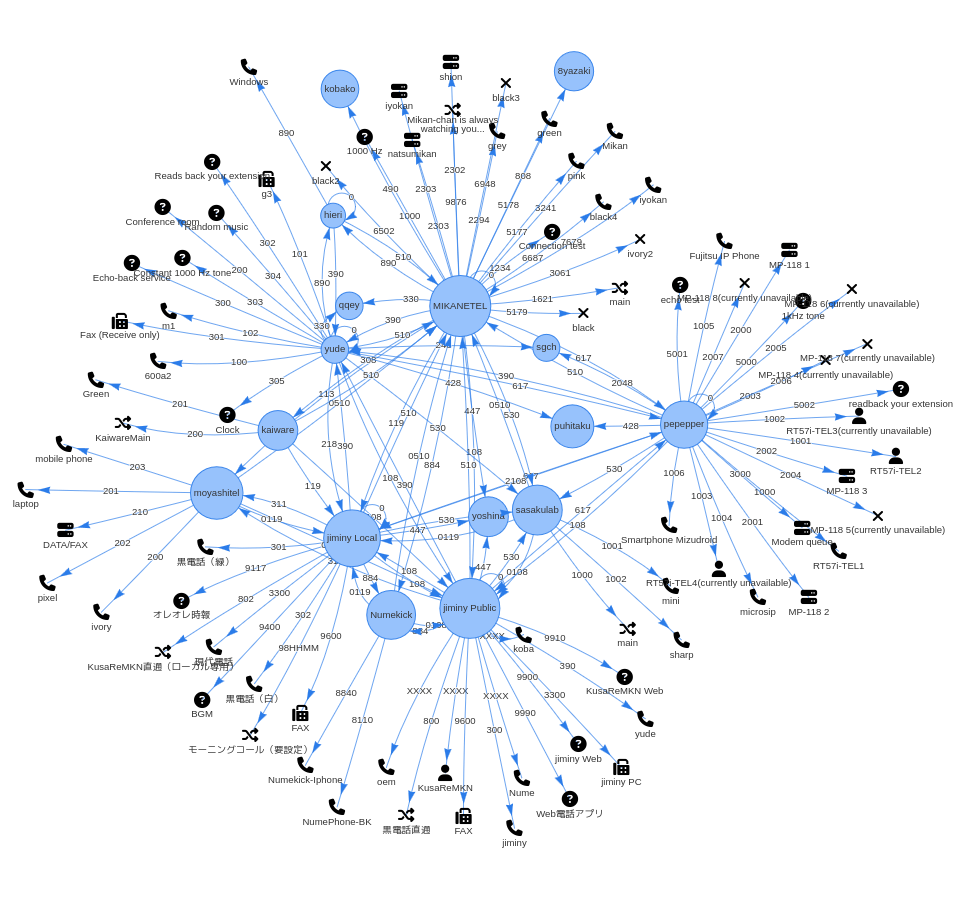
\includegraphics[height=.88\textheight]{./images/mantela.png}
    \end{column}
  \end{columns}

  \note{
    東京広域電話網の現在の姿を図に示すとこんな感じになるよ。
    ネットワークが複雑でちょっと見づらいのは許してね。
  }
\end{frame}

\begin{frame}
  \frametitle{東京広域電話網コミュニティ}

  \begin{description}[labelwidth=\linewidth]
    \item[Website]
      {\small
      \url{https://tkytel.github.io/}}
    \item[VRChat Group]
      {\small
      \href{https://vrc.group/TKYTEL.6282}{TKYTEL.6282}}
    \item[Discord]
      {\small
      \url{https://discord.com/invite/QEzAnuSy9S}}
    \item[GitHub Organization]
      {\small
      \url{https://github.com/tkytel}}
    \item[Mailing list]
      {\small
      \url{https://groups.google.com/g/tkytel}}
  \end{description}
  \note{
    東京広域電話網のコミュニティがあるよ。
    気軽に参加してみてね。
    VRChat Groupもできたよ!
  }
\end{frame}

\begin{frame}
  \frametitle{技術的なおはなし}

  \begin{description}[labelwidth=\linewidth]
    \item[いまさらVoIP網]
      {\small
      \url{https://zenn.dev/kusaremkn/articles/abd760f9f2f450}}
    \item[VoIPルータを使って黒電話をIP電話機にする]
      {\small
      \url{https://zenn.dev/kusaremkn/articles/187222dc1d4f1d}}
    \item[ICOM VE-TA10を使うためにパケットを書き換えたりする]
      {\small
      \url{https://zenn.dev/kusaremkn/articles/cb32b500fc1334}}
    \item[AudioCodes MP-118 VoIP GatewayをMikoPBXに収容する]
      {\small
      \url{https://zenn.dev/pepepper/articles/b8ad94b4b6f05f}}
  \end{description}
  \note{
    いまさらVoIP網でGoogleすると引っ掛かるハズなので、
    でんわをしてみたい人は検索してみてね。
    ほかにもいろいろあるよ。
  }
\end{frame}

\section{東京広域電話網の電話局同士の接続}
\note{
  東京広域電話網における電話局同士の接続について簡単に説明するよ。
}

\begin{frame}
  \frametitle{基本の構成}

  \begin{columns}
    \begin{column}{.6\textwidth}
      交換局として\textbf{MikoPBX}を用いる\\
      \hspace{1.5\zw}AsteriskベースのIP PBXシステム
      \\~\\[-.5\baselineskip]

      \textbf{Proxmox}や\textbf{Docker}を利用して\\
      \hspace{1.5\zw}コンテナ環境を構築
      \\~\\[-.5\baselineskip]

      交換局同士の相互接続には\\
      \hspace{1.5\zw}VPNサービス\textbf{Tailscale}を用いる
    \end{column}
    \begin{column}{.39\textwidth}
      
\includegraphics[width=\linewidth]{./images/mikopbx.png}
      \\~\\

      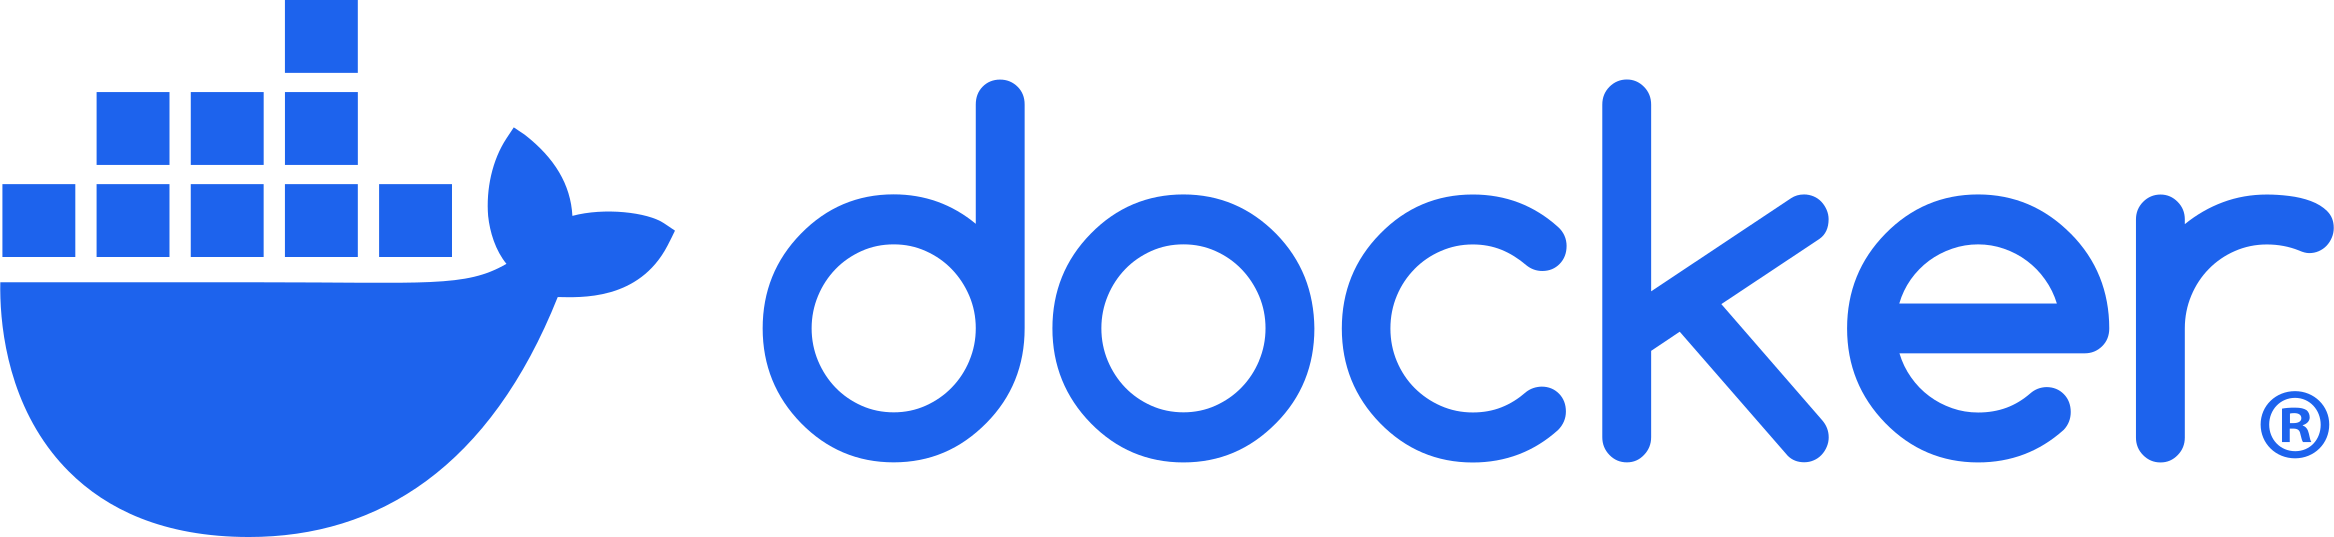
\includegraphics[width=\linewidth]{./images/docker.png}
      \\~\\

      
\includegraphics[width=\linewidth]{./images/tailscale.png}
    \end{column}
  \end{columns}
  \note{
    東京広域電話網の交換局の多くは、
    MikoPBXというAsteriskベースのIP PBXシステムを利用しているよ。
    MikoPBXを動作させる環境を構築するために
    ProxmoxやDockerなどのコンテナ仮想化技術を利用しているよ。
    また、網内の他の交換局と相互に接続するために、
    メッシュ形のVPNサービスであるTailscaleを利用しているよ。
  }
\end{frame}

\begin{frame}
  \frametitle{システム構成図}

  \includegraphics[page=4,width=\linewidth]{./images/pictures.pdf}

  \note{
    システム構成を簡単な図に表すとこのようになるよ。
    Ubuntuなど適当なホスト環境の上にDocker環境を用意し、
    その上でMikoPBXを動作させているよ。
    また、それぞれの局を接続するためにTailnetに接続しておくよ。
  }
\end{frame}

\begin{frame}
  \frametitle{交換局をホップするような通話にも対応}

  \includegraphics[page=7,width=\linewidth]{./images/pictures.pdf}
  \note{
    東京広域電話網では直接相互接続されていないような局同士でも
    通信できる仕組みを用意しているよ。
    これを交換局ホップと呼んでいるよ。
    交換局ホップを利用すると、
    直接相互接続されていないような局間の通信であっても、
    別の局を踏み台にして通信を実現することができるよ。
  }
\end{frame}

\section{網内のセキュリティ強化(素振り)}
\note{
  ここまで東京広域電話網の概要についてお話してきたので、
  ここから本編を始めていくよ。
}

\begin{frame}
  \frametitle{電話網内のセキュリティを向上しよう}

  東京広域電話網も最初は身内向けの小規模電話網だった\\
  \hspace{1.5\zw}網内のユーザは全員信頼されていることが前提
  \\~\\[-.5\baselineskip]

  時代は変わって大規模電話網になってしまった\\
  \hspace{1.5\zw}網内に悪意を持ったユーザが登場するおそれが出てきた\\
  \hspace{1.5\zw}(東京広域電話網はお前らを信じていますよ)
  \\~\\[-.5\baselineskip]

  → 網内のセキュリティを向上するための施策が必要

  \note{ }
\end{frame}

\begin{frame}
  \frametitle{懸念事項: Tailscaleでホストを共有している}

  電話局を相互接続するためにTailscaleを利用\\
  \hspace{1.5\zw}基本的には電話局のホストそれ自体を共有\\
  \hspace{1.5\zw}何もしていないとそのホストの全てが見える
  \\~\\[-.5\baselineskip]

  例えば……\\
  \hspace{1.5\zw}他局のMikoPBXの設定画面(Web UI)にアクセスできる\\
  \hspace{1.5\zw}MikoPBXをホストしているコンテナにSSHできる
  \\~\\[-.5\baselineskip]

  なんかちょっと怖そう(かなり怖そう)

  \note{ }
\end{frame}

\begin{frame}
  \frametitle{Tailscaleを使っているのだからTailscale ACLを使おう}

  Tailscale ACL(Access Control List)とは\\
  \hspace{1.5\zw}Tailnet上でアクセス制御をする手段
  \\~\\[-.5\baselineskip]

  Deny for defaultからアクセス許可するルールを列挙する\\
  \hspace{1.5\zw}初期状態では全アクセスを許可するルールを設定済

  \note{ }
\end{frame}

\begin{frame}
  \frametitle{とりあえず東京広域電話網の二大巨頭で実験}

  yude局及びMikaNeTEL局に設定して試験運用\\
  \hspace{1.5\zw}……が、なんかうまくいかない\\
  \hspace{1.5\zw}挙句の果てにはyude-MikaNeTEL間の通信ができなくなる\\
  \hspace{1.5\zw}→ 交換局ホップに頼っている経路に影響
  \\~\\[-.5\baselineskip]

  全てを元に戻してほぼ初期状態へ\\
  \hspace{1.5\zw}MikoPBXに付属しているFirewallを利用する方針へ変更\\
  \hspace{1.5\zw}コンテナをhostモードで運用しているためこれで良かった

  \note{ }
\end{frame}

\section{不思議な不通問題}
\note{ }

\begin{frame}
  \frametitle{新規局参入 → 不通}

  いつものように東京広域電話網に新規局が参入\\
  \hspace{1.5\zw}接続確認のための自動応答番号を設置しがち\\
  \hspace{1.5\zw}ノウハウがぼんやりとしているのでたびたび事故が起きる
  \\~\\[-.5\baselineskip]

  例によって今回も確認用の番号に掛けるも無音\\
  \hspace{1.5\zw}よくあるトラブルシューティングのノリで対応開始\\
  \hspace{1.5\zw}設定項目を確認するもこれといって問題点は見付からず\\
  \hspace{1.5\zw}どうしようもないので人対人通信で接続を確認することに

  \note{ }
\end{frame}

\begin{frame}
  \frametitle{前例のない不具合: ベルは鳴れど通話はできず}

  相手に電話を掛けると「プルプルプル」の音が鳴る\\
  \hspace{1.5\zw}電話の受け側でもベルが鳴っている
  \\~\\[-.5\baselineskip]

  相手が受話器を上げたらしく「プルプルプル」の音が止む\\
  \hspace{1.5\zw}とりあえず「もしもし」してみる\\
  \hspace{1.5\zw}電話の受け側では「もしもし」が聞こえる\\
  \hspace{1.5\zw}しかし返事は聞こえない(しばらくすると通話が切れる)

  \note{ }
\end{frame}

\begin{frame}
  \frametitle{IP電話のウラ側: 呼制御のSIPと実通信のRTP}

  \begin{columns}
    \begin{column}{.35\textwidth}
      ベルが鳴っている\\
      \hspace{1\zw}→ SIPはOKっぽい
      \\~\\[-.5\baselineskip]

      声が聞こえない\\
      \hspace{1\zw}→ RTPが死んでる
      \\~\\[-.5\baselineskip]

      勝手に通話が切れる\\
      \hspace{1\zw}→ だんまりだから
    \end{column}
    \begin{column}{.65\textwidth}
      \raggedleft
      ~\\[.2\baselineskip]
      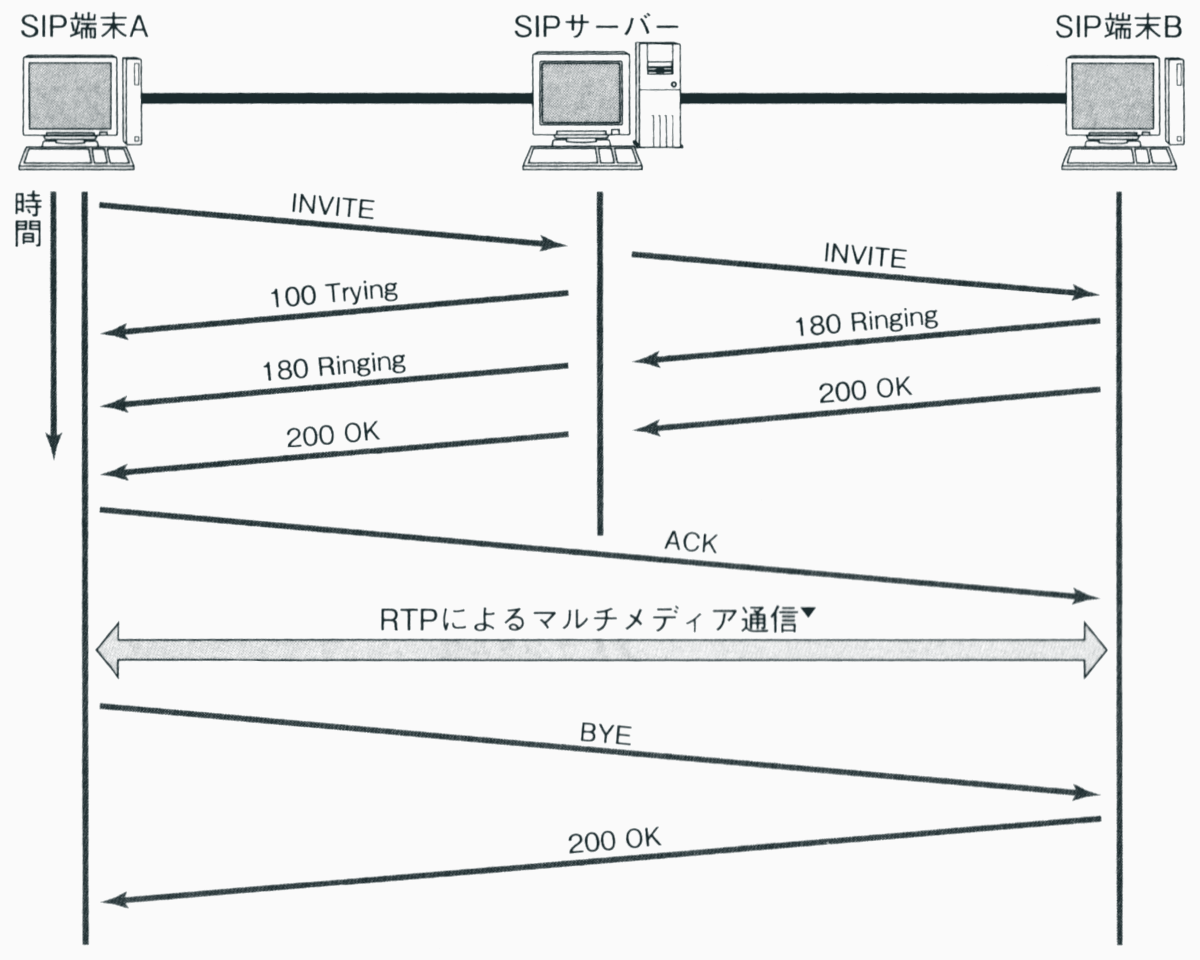
\includegraphics[height=.9\textheight]{./images/sip.png}
    \end{column}
  \end{columns}

  ~\\[-.9\baselineskip]
  {\tiny\raggedright
  井上直也,村山公保,竹下隆史,荒井 透,苅田幸雄:\\[-1.5\baselineskip]
  \raggedright
  第8章 アプリケーションプロトコル,
  「マスタリングTCP/IP 入門編(第6版)」,
  p.334,
  株式会社オーム社,2021.}
  \\~\\[3\baselineskip]

  \note{ }
\end{frame}

\begin{frame}
  \frametitle{どうしてSIPは届いてRTPは届かないのか}

  Firewallか何かが悪さをしていそう\\
  \hspace{1.5\zw}この局はTailscale ACLやMikoPBX Firewallをいじっていた\\
  \hspace{1.5\zw}Tailscale ACLはyude-MikaNeTEL間のことで嫌になっている
  \\~\\[-.5\baselineskip]

  いったん全ての武装を解除してみる\\
  \hspace{1.5\zw}Tailscale ACLをall allowに\\
  \hspace{1.5\zw}MikoPBX Firewallをdisabledに\\
  \hspace{1.5\zw}しかし改善せず(は?)→ 泥沼のスタート

  \note{ }
\end{frame}

\begin{frame}
  \frametitle{調べてみると片方向通信になる話が出てくる}

  NAPT環境下だと片方向通信になりがち\\
  \hspace{1.5\zw}NAPT環境で外から内に入ってくるには\\
  \hspace{1.5\zw}能動的に内から外に出る必要がある
  \\~\\[-.5\baselineskip]

  SIPの通信はこれに該当する\\
  \hspace{1.5\zw}SIPサーバはリクエストがあって初めて答えてくれる
  \\~\\[-.5\baselineskip]

  RTPの通信はこれに該当しない\\
  \hspace{1.5\zw}SIP上で指定されたポートを狙って勝手に飛んでくる\\
  \hspace{1.5\zw}NAPTは飛んできたパケットを誰に転送するのかわからない

  \note{ }
\end{frame}

\begin{frame}
  \frametitle{や、でもこれTailnet内の通信だよ?}

  あ、そうだったわ

  \note{ }
\end{frame}

\begin{frame}
  \frametitle{その他の関係ない人たち}

  上流がRakuten Turbo 5Gルータだよ?\\
  \hspace{1.5\zw}→ 同様の環境で疎通してる別の局がありました
  \\~\\[-.5\baselineskip]

  無線だからかRTTめちゃくちゃデカいよ?\\
  \hspace{1.5\zw}→ バカ遅いリンクでも他局と通信できました(10Base2)
  \\~\\[-.5\baselineskip]

  音声コーデック非対応なんじゃない?\\
  \hspace{1.5\zw}→ よく使われるものに絞ってもダメでした

  \note{ }
\end{frame}

\section{ええい、総当たりじゃ!}
\note{ }

\begin{frame}
  \frametitle{とりあえず全局と接続テストしてみる}

  東京広域電話網の全ての局で片方向通信になるのか確かめてみる\\
  \hspace{1.5\zw}通信できる局は比較的多かった\\
  \hspace{1.5\zw}むしろ片方向通信や不通になる方がレア
  \\~\\[-.5\baselineskip]

  通信できる他の局をホップしてから通信すると繋がる\\
  \hspace{1.5\zw}これに頼っても良いけどちょっと不便かも\\
  \hspace{1.5\zw}(スケールできないことを露呈していてダメ)
  \\~\\[-.5\baselineskip]

  とはいえ、原因となるものが何もわからない

  \note{ }
\end{frame}

\begin{frame}
  \frametitle{伝家の宝刀 パケットキャプチャ}

  \texttt{tcpdump}を使ってパケットを眺めてみる\\
  \hspace{1.5\zw}SIPのパケットは問題なさそうに見える\\
  \hspace{1.5\zw}予想通りRTPのパケットは片方しか来ていない
  \\~\\[-.5\baselineskip]

  しかもなんか変なNICに出てる\\
  \hspace{1.5\zw}tailnet上の通信は仮想NIC(\texttt{tialscale0})に流れるハズ\\
  \hspace{1.5\zw}発狂している通信では物理NIC(\texttt{eth0})に流れている

  \note{ }
\end{frame}

\begin{frame}
  \frametitle{あぁ、ちゃんと100.70.198.29にパケット投げてるのに!}

  「え、100.67.198.29って誰ですか」
  \\~\\[2\baselineskip]

  「は?」

  \note{ }
\end{frame}

\begin{frame}
  \centering
  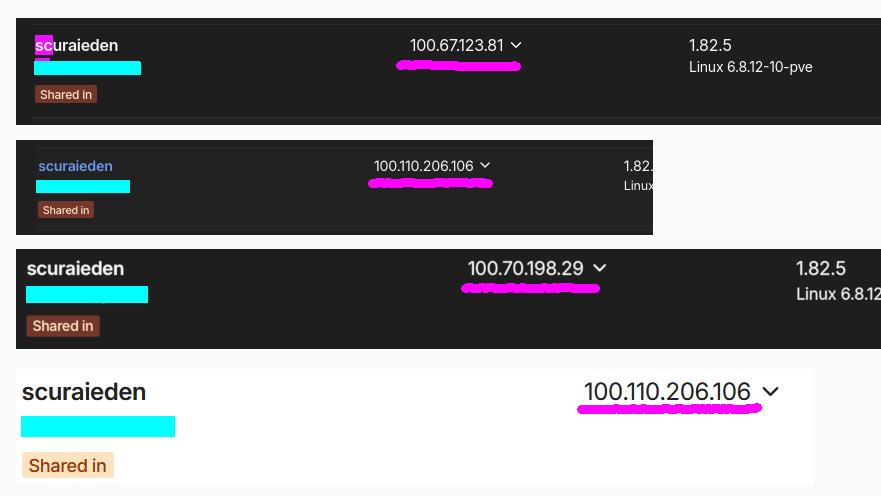
\includegraphics[height=.9\textheight]{./images/hakkyo.png}
\end{frame}

\begin{frame}
  \frametitle{TailscaleでIPv4アドレスを割り当て直すと通信可能に!}

  Tailscaleの機能でIPv4アドレスを再設定\\
  \hspace{1.5\zw}通信の両端で同じアドレスとなるように設定\\
  \hspace{1.5\zw}無事に通信できるようになりました
  \\~\\[-.5\baselineskip]

  \hfill ……本当か?

  \note{ }
\end{frame}

\section{考察・追実験}
\note{ }

\begin{frame}
  \frametitle{互いに異なるIPv4アドレスが見えていたため発狂した?}

  お互いに見えているIPv4アドレスが異なる事象\\
  \hspace{1.5\zw}Tailscaleがよしなにしているなら問題ないハズ\\
  \hspace{1.5\zw}つまり、TailscaleがNATのように仕事をしている?

  SIPで通信できたのはNAT的ふるまいのおかげ

  RTPはSIPで指定されたIPアドレス・ポートを使う\\
  \hspace{1.5\zw}指定された場所は存在しないのでルーティングで発狂\\
  \hspace{1.5\zw}実行環境のLinuxも混乱して\texttt{eth0}にパケットぶん投げる

  \note{ }
\end{frame}

\begin{frame}
  \frametitle{じゃあ追実験だ!}

  通信できている局間でIPv4アドレスを変えたら発狂するのか

  \begin{itemize}
    \item[1.]
      通信できている局の対を用意する
    \item[2.]
      片方のIPv4アドレスを変更してみる(発狂させる)
    \item[3.]
      通信が壊れる
    \item[4.]
      IPv4アドレスを直したら通信できるようになる
  \end{itemize}

  \note{ }
\end{frame}

\begin{frame}
  \frametitle{実験は失敗しました}

  \begin{itemize}
    \item[1.]
      通信できている局の対を用意する
    \item[2.]
      片方のIPv4アドレスを変更してみる(発狂させる)
    \item[3.]
      \dsout{通信が壊れる} ← \textbf{壊れませんでした}
    \item[4.]
      IPv4アドレスを直したら通信できるようになる
  \end{itemize}

  そもそも異なるIPv4アドレスが見えていたのに\\
  \hspace{1.5\zw}通信できていた局も存在していたのでした(何もわからん)

  \note{ }
\end{frame}

\section{まとめ}
\note{ }

\begin{frame}
  \frametitle{オレオレIP電話網を破壊したり発狂したりしてみた}

  分散形の異常オレオレIP電話網「東京広域電話網」

  ベルは鳴るのに音声が届かない問題を掘り下げた

  SIPとRTPとの通信の違いを確認した

  Tailscaleのせいなのか何なのかよくわからない感じになった

  ~\\[-.5\baselineskip]

  バックボーンの通信も自分で実現すれば発狂せずに済むかもネ\\
  \hspace{1.5\zw}東京広域通信網に乞うご期待
\end{frame}

\begin{frame}[standout]
  おわりです
  \note{
    発表おわり〜
  }
\end{frame}

\begin{frame}
  \frametitle{このスライドについて}

  Written in May 2025.
  \\~\\[-.5\baselineskip]

  Permanent ID of this document: \texttt{c8edfb391dbbafd3}.
  \\~\\[-.5\baselineskip]

  Copyright © 2025 KusaReMKN, 東京広域電話網.
  \\~\\[-.5\baselineskip]

  特記無き場合、プログラムやソースコードは MIT License で、\\
  \hspace{1.5\zw}それ以外のコンテンツは CC-BY 4.0 で利用可能です。\\
  \hspace{1.5\zw}一部の画像には別のライセンスが適用されるかもしれません。
\end{frame}



%%%%%%%%%%%%%%%%%%%%%%%%%%%%%%%%%%%%%%%%%%%%%%%%%%%%%%%%%%%%%%%%%%%%%%%%%%%%%%%
\appendix

\begin{frame}[standout]
  ここから前回のスライド
  \note{ }
\end{frame}

\title{世も令和になって久しいので\\オレオレIP電話網や黒電話で遊んでみる\\(再放送版)}
\subject{CS集会\#47}
\author{上羽 未栞(a.k.a. KusaReMKN)}
\institute{%
  \url{https://KusaReMKN.com/}\\
  Twitter: \href{https://twitter.com/KusaReMKN}{@KusaReMKN}}
\keywords{黒電話; VoIP; IP電話; MikoPBX; 東京広域電話網}
\date{2025-03-11}

\begin{frame}
  \titlepage
  \note{
    発表を始めるよ。

    「世も令和になって久しいのでオレオレIP電話網や黒電話で遊んでみる」と題して、
    みかんちゃんが発表するよ。
  }
\end{frame}

\begin{frame}
  \frametitle{今回のおはなし}

  ~\\[-.25\baselineskip]
  \tableofcontents
  \note{
    今回の発表の流れはこんな感じだよ。
    質疑応答を含めて大体25分間くらいで進められたらいいな。
  }
\end{frame}

\section*{みかんちゃんについて}
\note{
  自己紹介するよ。
}

\begin{frame}
  \frametitle{自称・大天才美少女プログラミング初心者}

  \begin{textblock*}{0.5\paperwidth}(0.6cm, 3.5cm)
    
\includegraphics[width=0.3\paperwidth]{./images/mikanchan.png}
  \end{textblock*}
  \begin{columns}
    \begin{column}{0.30\textwidth}
      \\~\\[-.25\baselineskip]
    \end{column}
    \begin{column}{0.69\textwidth}
      \\~\\[-.25\baselineskip]
      「\ruby{上羽}{うわ|ば} \ruby{未栞}{み|かん}」
      あるいは「\ruby[g]{KusaReMKN}{くされみかん}」\\
      \hspace{1.5\zw}\textbf{みかんちゃん}って呼んでね!
      \\~\\[-.5\baselineskip]

      \newlength{\zeropeke}
      \settowidth{\zeropeke}{\tiny 0x}
      \hspace{-\zeropeke}{\tiny 0x}18\nobreak 歳のJK(重要)
      \\~\\[-.5\baselineskip]

      実はプログラマでもエンジニアでもない\\
      \hspace{1.5\zw}古い計算機っぽいものが大好き
      \\~\\[-.5\baselineskip]

      Twitterで思想を垂れ流すことが得意\\
      \hspace{1.5\zw}\url{https://kusaremkn.com/}も見てね
    \end{column}
  \end{columns}
  \note{
    大天才美少女プログラミング初心者を自称している、上羽未栞だよ。
    みかんちゃんって呼ばれると大変喜ぶよ。
    イチハチ歳のJKだよ。

    大天才とかプログラミング初心者とか言っているけれど、
    実はプログラマでもエンジニアでもないよ。
    外の人(学生のすがた)は通信方式について研究していたりするけれど、
    それはまた別のお話だよ。
    それはそれとして古い計算機っぽいものが大好きだよ。
    よくハードオフに出没してジャンク箱を小豆洗いしているよ。

    Twitterとかウェブサイトとかあるよ。
    暇な人は覗いてみてね。
    深淵があるよ。
  }
\end{frame}

\section{「でんわ」のはじまり}
\note{
  早速「でんわ」についてお話していくよ。
}

\begin{frame}
  \frametitle{HARD OFFに売られていた黒電話(白色)}

  \centering
  \includegraphics[height=.85\textheight]{./images/ivory.jpeg}
  \note{
    いつものようにハードオフをふらついていると黒電話(白色)が現れたよ。
    最初はにらめっこをしているだけだったんだけど、
    気付いたら財布の中身が軽くなって手元に電話機が発生していたよ。
    これがみかんちゃんと「でんわ」との邂逅だよ。
  }
\end{frame}

\begin{frame}
  \frametitle{一方そのころ、限界セルフホスティング界隈では……}

  \begin{columns}[c]
    \begin{column}[c]{.80\textwidth}
      \ruby[g]{\bfseries MMTNET}{ももたねつと}:\\
      \hspace{1.5\zw}Malleable Mutual Tunneling Network\\
      \hspace{1.5\zw}for Experimental Technologies
      \\~\\[-.5\baselineskip]

      SoftEther VPNを使ってホストを相互接続\\
      \hspace{1.5\zw}自作インターネットを目論んでいた
      \\~\\[-.5\baselineskip]

      MMTNET上で動作するアプリケーション\\
      \hspace{1.5\zw}黒電話を利用したIP電話が挙げられていた\\
      \hspace{1.5\zw}MMTNETの前身(HVCAN)でも運用されていた
    \end{column}
    \begin{column}{.17\textwidth}
      \centering
      \\~\\[-.75\baselineskip]
      
\includegraphics[width=\linewidth]{./images/pepepper.jpg}

      
\includegraphics[width=\linewidth]{./images/yude.jpg}

      
\includegraphics[width=\linewidth]{./images/kurari.jpg}
    \end{column}
  \end{columns}
  \note{
    みかんちゃんが「でんわ」と邂逅している一方、
    限界セルフホスティング界隈(スライド右側の人々)では
    MMTNETとかいうけしからんネットワークが構築されようとしていたよ。
    MMTNETはSoftEther VPNを利用したネットワークで、
    この上で自作のインターネットを作ることを目論んでいたよ。

    このMMTNET上で動作するアプリケーションとして、
    黒電話を利用したIP電話が挙げられていたよ。
    これはどういうことかというと、
    MMTNETの前身にあたるネットワークとして
    HVCANという異常ネットワークがあるんだけど、
    これの上で黒電話IP電話が実現していたので、
    これをもっと発展させてみよいうという話だったよ。
  }
\end{frame}

\begin{frame}
  \frametitle{HVCAN上のIP電話発足の貴重なシーン}

  ~\\[-.75\baselineskip]
  \begin{columns}[b]
    \begin{column}{.49\textwidth}
      \centering
      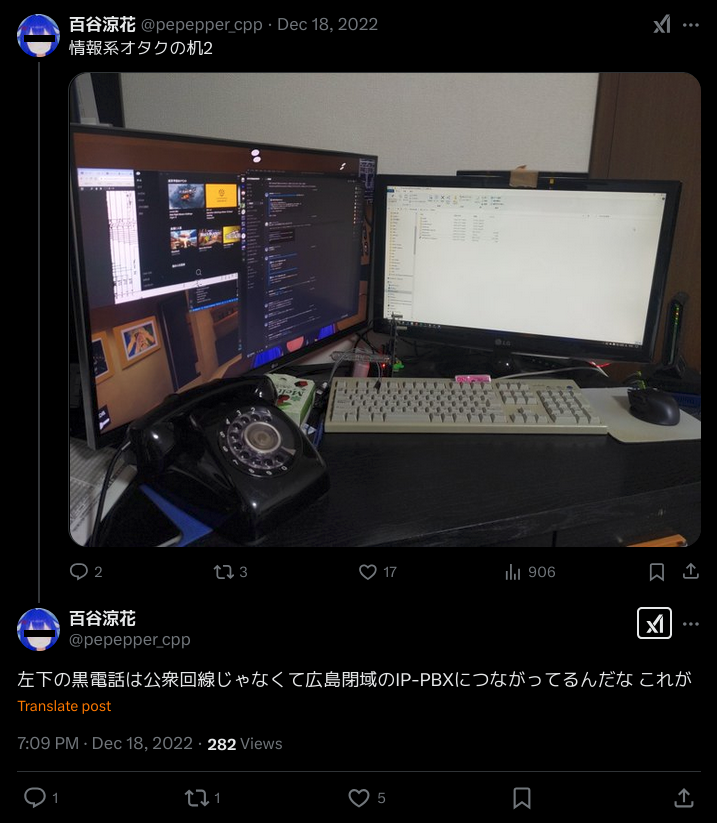
\includegraphics[height=.9\textheight]{./images/ijyou.png}
    \end{column}
    \begin{column}{.49\textwidth}
      \centering
      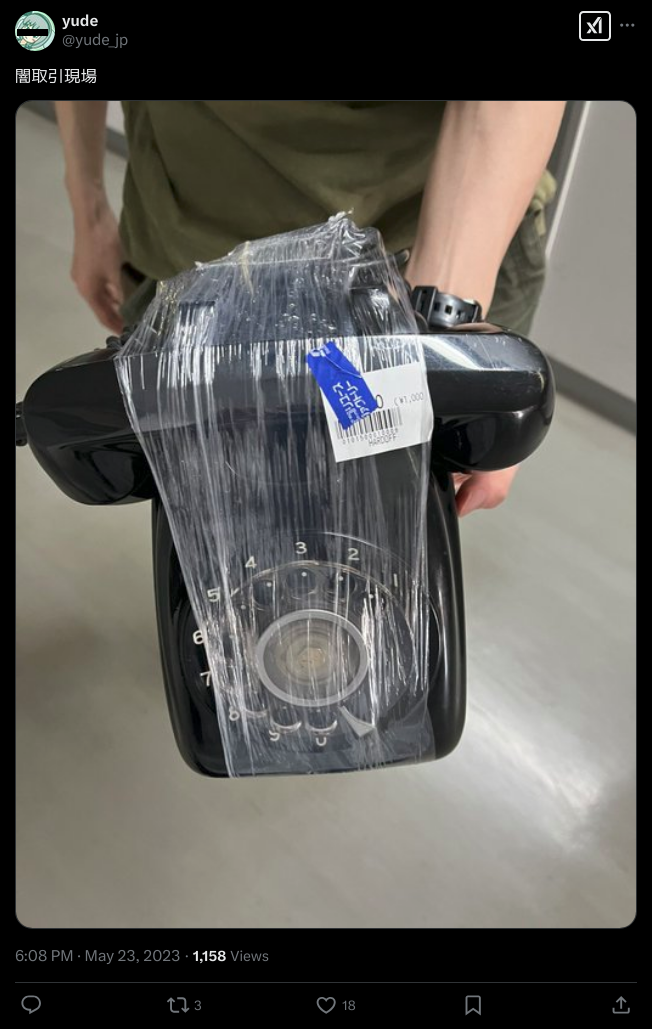
\includegraphics[height=.9\textheight]{./images/yami.png}
    \end{column}
  \end{columns}
  \note{
    HVCANでIP電話が実現されていたことを確認するためにツイートを遡ってみたよ。
    うん、確かに異常オタクの机に黒電話は存在しているし、
    しかもハドフで得た黒電話を取引している怪しい現場写真まで出てきたよ。
  }
\end{frame}


\begin{frame}
  \frametitle{HVCAN上の電話網(?)の様子}

  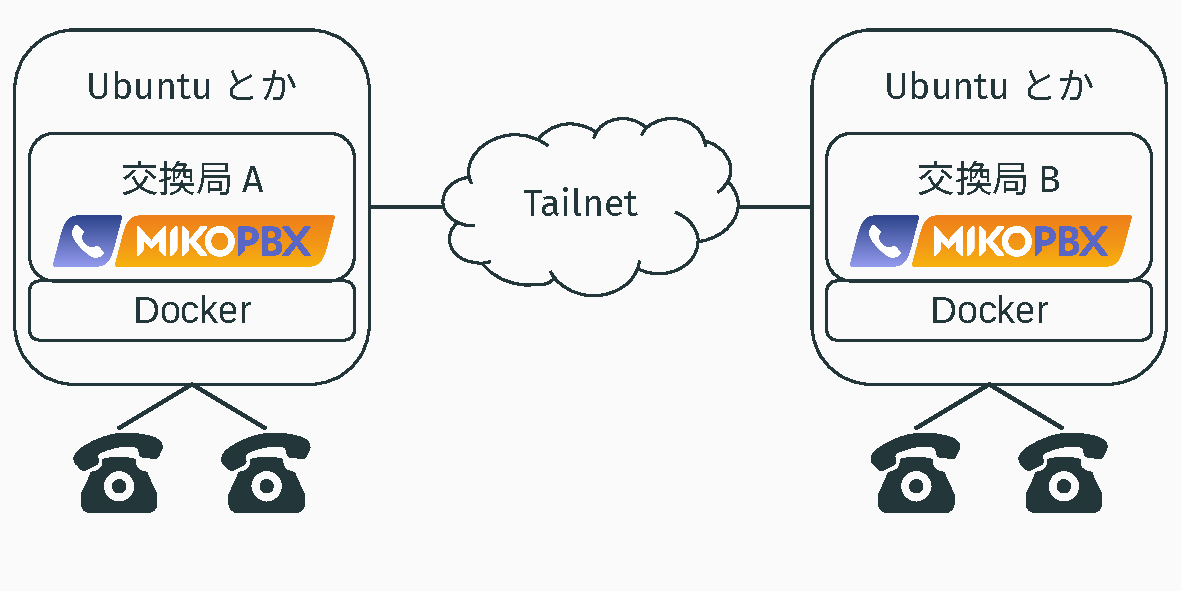
\includegraphics[page=1,width=\linewidth]{./images/pictures.pdf}
  \note{
    HVCANの上で実現していたIP電話のシステムを図に起こすとこんな感じになるよ。
    HVCANには単一の交換局があって、
    これに全ての端末(電話機)が接続されていたよ。
    つまり、事実上の内線電話に留まっていたよ。
  }
\end{frame}

\begin{frame}
  \frametitle{実現したいこと}

  \begin{description}[labelwidth=\linewidth,itemsep=.25\zh]
    \item[外線通話と多局接続]
      交換局をまたぐ通話\\
      複数の交換局の相互接続
    \item[交換局ホップ]
      相互接続されていない局の通話
  \end{description}

  状況を簡単にするためMMTNETから切り離される\\
  \hspace{1.5\zw}オレオレ電話網「\textbf{東京広域電話網}」の爆誕
  \note{
    というわけで、今回実現したいことは次の二つだよ。
    一つ目は外線通話、多局接続の実現だよ。
    これは交換局をまたぐような通話であったり、
    沢山の交換局が相互に接続された電話網を構築したりする部分にあたるよ。
    二つ目は交換局ホップだよ。
    後のスライドでも述べるけれども、
    交換局が増えてくると全ての局を直接相互接続することが現実的ではなくなってくるよ。
    これを解決するために、直接接続されていない局同士でも通話できるようにするよ。

    これがMMTNET上にあると、多くの人類のためにならないよ。
    多くの人間はMMTNET上にいないからだよ。
    そのため、MMTNETから電話網の部分を切り出して電話網単体の問題として解決することにしたよ。
    オレオレ電話網「東京広域電話網」が爆誕したよ。
  }
\end{frame}

\section{外線通話と多局接続}
\note{
  一つ目の問題である外線通話と多局接続について考えるよ。
}

\begin{frame}
  \frametitle{基本の構成}

  \begin{columns}
    \begin{column}{.6\textwidth}
      交換局として\textbf{MikoPBX}を用いる\\
      \hspace{1.5\zw}AsteriskベースのIP-PBXシステム\\
      \hspace{1.5\zw}シンプルなWEB UIが魅力
      \\~\\[-.5\baselineskip]

      スタンドアロン版とDocker版がある
    \end{column}
    \begin{column}{.39\textwidth}
      
\includegraphics[width=\linewidth]{./images/mikopbx.png}
    \end{column}
  \end{columns}
  \note{
    まずは交換局の構成について説明するよ。
    今回の電話網構築にはフリーのPBXシステムであるMikoPBXを用いるよ。
    これはAsteriskというIP-PBX(要はIP電話の交換局システム)をベースとしたシステムだよ。
    シンプルなWEB UIが魅力だよ
    (つまり他のPBXシステムにはシンプルでないWEB UIをもつものがあるということだよ)。
    MikoPBXにはスタンドアロン版とDocker版があるので使い分けられるよ。
  }
\end{frame}

\begin{frame}
  \frametitle{ダメなシステム構成(その1)}

  \includegraphics[page=2,width=\linewidth]{./images/pictures.pdf}
  \note{
    まずはスタンドアロン版を使うことを考えてみるよ。
    これが最も簡単な構成であるのだけれど、
    これはちょっとむつかしくて、
    交換局はグローバルなインターネットに晒されなければならないよ。
    セキュリティ的にも嫌な気持ちになるし、
    そもそも全ての局がグローバルなIPアドレスを持たなければならなくて、
    現実的じゃないね。
  }
\end{frame}

\begin{frame}
  \frametitle{VPNを使えばいいじゃない}

  \begin{columns}
    \begin{column}{.6\textwidth}
      交換局間の接続に\textbf{Tailscale}を用いる\\
      \hspace{1.5\zw}簡単なメッシュ型VPNサービス\\
      \hspace{1.5\zw}ユーザ間で接続を共有できてお得
    \end{column}
    \begin{column}{.39\textwidth}
      
\includegraphics[width=\linewidth]{./images/tailscale.png}
    \end{column}
  \end{columns}
  \note{
    インターネットに晒すことが問題であるならば、
    VPNを使えばこの問題を解決できそうだよ。
    今回はTailscaleを使うことを考えたよ。
    Tailscaleは大変すばらしいメッシュ型のVPNサービスだよ。
    みんなも使ったことあるかも(?)
    ユーザ内のVPNを作ることもできるし、
    VPN上のホストを他のユーザと共有できたりしてお得だよ。
  }
\end{frame}

\begin{frame}
  \frametitle{ダメなシステム構成(その2)}

  \includegraphics[page=3,width=\linewidth]{./images/pictures.pdf}
  \note{
    なるほど、Tailscaleを使えば完璧だ、と思ったけどやっぱりこれもダメだったよ。
    スタンドアロン版のMikoPBXはLinuxディストリみたいに
    完結したシステムとして提供されるのだけれど、
    この上でTailscaleのクライアントソフトを動かせそうにないことがわかったよ。
    クライアントソフトが動かないとTailscale越しの接続を実現できるハズもないので、
    これではいけないね。
  }
\end{frame}

\begin{frame}
  \frametitle{Docker版を使えばいいじゃない}

  \begin{columns}
    \begin{column}{.6\textwidth}
      \textbf{Docker}版MikoPBXを用いる\\
      \hspace{1.5\zw}ホスト側でTailnetに接続\\
      \hspace{1.5\zw}MikoPBX側は何も考えなくてよい
    \end{column}
    \begin{column}{.39\textwidth}
      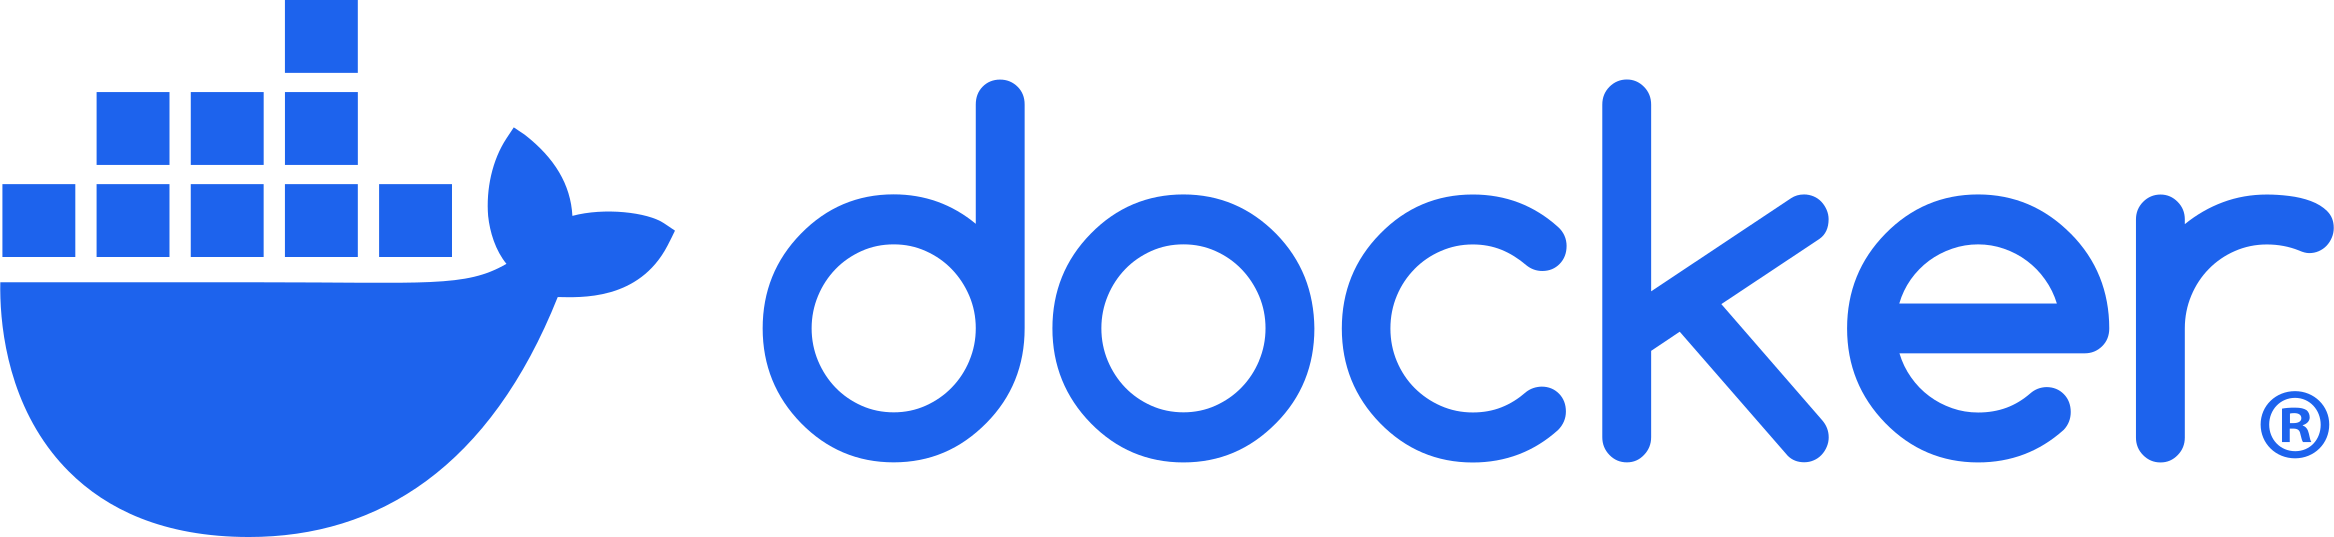
\includegraphics[width=\linewidth]{./images/docker.png}
    \end{column}
  \end{columns}
  \note{
    ところで、ちょっと思い出してみるとMikoPBXにはDocker版があったね。
    これを使うと簡単に構成できそうだよ。
    Dockerコンテナを動かすホスト環境(これは普通Ubuntuだよ)で
    Tailscaleのクライアントソフトを動かすことは容易いよ。
    この環境の上に構築されるMikoPBXは
    当然Tailscaleのネットワークに接続できるので、
    特段むつかしいことを考える必要がないよ。
  }
\end{frame}

\begin{frame}
  \frametitle{完成版のシステム構成}

  MikoPBXの設定をこねくり回していたら外線通話が可能に!

  \includegraphics[page=4,width=\linewidth]{./images/pictures.pdf}

  \note{
    というわけで完成版のシステム構成がこんな感じだよ。
    Ubuntuとかの上にTailscaleをインストールして
    Tailnet経由で接続できるようにしておくよ。
    この上にDocker環境を用意して、
    その上にDocker版のMikoPBXをインストールするよ。

    この構成にして、
    MikoPBXの設定をこねくり回すこと二三日していたら外線接続が実現できたよ。
    (東京と横浜との交換局が繋がったときみたいな感動があるね(は?))

    (2024-11-11)
  }
\end{frame}

\begin{frame}
  \frametitle{内線接続に加え、外線接続もできるようになった!}

  \vspace{\baselineskip}
  \includegraphics[page=8,width=\linewidth]{./images/pictures.pdf}

  \note{
    これまでできていた同一局内の端末同士の内線通話に加えて、
    局をまたいで別の局の端末との通話(外線通話)もできるようになったよ。
  }
\end{frame}

\begin{frame}
  \frametitle{多局接続がむつかしい}

  \includegraphics[page=5,width=\linewidth]{./images/pictures.pdf}
  \note{
    さて、外線通話の実現はできたわけだけれども、
    多数の交換局が相互に接続できるようになるには少しだけ時間が掛かったよ。
    というのも、局Aと局Bとがあってこれらが接続済のときに、
    局Cが局Aに接続しようとするとなぜか拒否されてしまうという問題が発生していたよ。
  }
\end{frame}

\begin{frame}
  \frametitle{WEBに表示されていない設定項目}

  \begin{columns}
    \begin{column}{.7\textwidth}
      MikoPBXのWEB UIで設定を変更すると\\
      \hspace{1.5\zw}システムの設定ファイルが書き変わる
      \\~\\[-.5\baselineskip]

      WEB UIに表示されていない項目もある\\
      \hspace{1.5\zw}設定項目\texttt{max\_contacts}\\
      \hspace{1.5\zw}デフォルトの値は\textbf{1}\\
      \hspace{1.5\zw}これを100にすると接続できる
    \end{column}
    \begin{column}{.29\textwidth}
      
\includegraphics[width=\linewidth]{./images/jiminy.jpg}
    \end{column}
  \end{columns}
  \note{
    この問題を解決する鍵はもっと下側の層にあったよ。
    MikoPBXのWEB UIで設定を変更すると、
    その下側で動作しているAsteriskシステムの設定ファイルが書き変わるよ。

    異常オタクがこれについてめちゃくちゃ調査をしたところ原因がわかったよ。
    設定項目のうち、システムの動作に関わるいくつかの項目はWEB UI上に表示されていなかったよ。
    この設定項目がmax\_contactsだよ。
    この項目のデフォルトの値は1で、つまり同時に接続を受ける局の数は1に制限されていたよ。
    設定ファイルを直接書き換えてこの値を100とか1000とかに変更すると接続できるようになったよ。
    これで電話「網」を構築できるようになったよ。(2024-11-23)
  }
\end{frame}

\section{交換局ホップ}
\note{
  次に二つ目の問題である交換局ホップについて考えるよ。
}

\begin{frame}
  \frametitle{新しい局を追加する際の手間}

  \includegraphics[page=6,width=\linewidth]{./images/pictures.pdf}
  \note{
    電話網を構築できることがわかると、電話網は急速に発展していったよ。
    ここで問題になってきたのが新しい電話局を追加するときの手間だよ。
    電話局は相互に接続されていないと通話ができなかったので、
    例えば局Fが新しく網A--Eに接続しようとすると、
    全ての局で設定を行う必要があったよ。
    これはもう大変面倒だし、
    今後の発展を考えると現実的ではないことが明らかになってきたよ。
    }
\end{frame}

\begin{frame}
  \frametitle{インターネットにできるなら電話網にもできる}

  インターネットのルータは完全グラフを構成していない\\
  \hspace{1.5\zw}それでも多くのホストと通信できる
  \\~\\[-.5\baselineskip]

  電話網の全ての局が完全グラフを構成していない場合\\
  \hspace{1.5\zw}局同士がよしなに通話を取り持ってくれれば\\
  \hspace{1.5\zw}直接接続されていない局間でも通話を実現できるのでは?
  \note{
    ここで、インターネットに思いを馳せてみると、
    インターネットの上側で仕事をしてくれているルータたちは
    完全グラフを構成していない
    (全てのルータが相互に直接接続されていない)ことがしばしばだよ。
    しかし、私達は不自由なくインターネットを使えているし、
    インターネット上のほとんどのホストと通信できるよ。
    どういう仕組みかというと、
    ルータがパケットをバケツリレーしてくれているので通信できるんだね。

    ところで、電話網でも交換局が完全グラフを構成してなくても、
    交換局がよしなに通話を取り持ってくれれば、
    直接接続されていない局同士でも通信できるんじゃないかな、と考えられるよ。
  }
\end{frame}

\begin{frame}
  \frametitle{電話を掛け直す電話番号}

  \begin{columns}
    \begin{column}{.7\textwidth}
      通常の外線着信の場合\\
      \hspace{1.5\zw}\textbf{着信局内の端末のみ}を対象に検索\\
      \hspace{1.5\zw}→ 再び\textbf{外線接続することはない}
      \\~\\[-.5\baselineskip]

      特定の番号に電話を掛けた場合\\
      \hspace{1.5\zw}番号を検索する部分でインチキをする\\
      \hspace{1.5\zw}\textbf{外線の番号}も検索しなおしてもらう\\
      \hspace{1.5\zw}→ 再び\textbf{外線接続のチャンスがやってくる}
    \end{column}
    \begin{column}{.29\textwidth}
      
\includegraphics[width=\linewidth]{./images/jiminy.jpg}
    \end{column}
  \end{columns}
  \note{
    これもまた異常オタクによって実現されたよ。

    通常の外線着信のルーティーンを覗いてみると、
    着信した局内の(つまり内線接続されている)端末のみを対象に
    番号を検索していることがわかったよ。
    内線番号のみを対象にしているので、
    外線番号が検索対象になることはないよ。

    ここで、特別な番号を用意してあげて、
    この番号では端末に接続するかわりにインチキ処理をすることにするよ。
    具体的には、この番号に続く番号を外線番号として解して
    検索しなおしてもらう処理にジャンプするよ。
    これによって外線接続を着信しても再び外線接続のチャンスがやってくるよ。
    つまり、着信局は外線に着信をバケツリレーできて、
    別の局に通話を取り次げるようになるよ。
  }
\end{frame}

\begin{frame}
  \frametitle{番号検索ルーティーン}

  \includegraphics[page=9,width=\linewidth]{./images/pictures.pdf}
  \note{
    番号検索ルーティーンのイメージをスライドに示しているよ。
    Asteriskのプログラムはgotoとgosubとの嵐で
    古いBASICを彷彿とさせる最悪さがあるよ。

    外線からの着信はちょっとだけ処理をされてから
    内線番号を検索する部分にジャンプしているよ。
    内線番号を検索する部分には
    ダイヤルプランアプリケーションや端末番号を検索する処理があるよ。
    ここで番号が見つからなかったら着信失敗になるよ。

    で、アプリケーションとしてフック用の番号を用意してあげて、
    そこから全ピア検索のルーティーンにジャンプするように細工をするよ。
    これによって外線着信から外線発信できるようになって、
    別の局に通話を取り次げるようになったよ。
  }
\end{frame}

\begin{frame}
  \frametitle{相互接続されていない局間でも通話が可能に}

  \includegraphics[page=7,width=\linewidth]{./images/pictures.pdf}
  \note{
    つまり、例えば、局Fが局Eに電話をかけたいときには、
    局Cを踏み台にして通話できるようになったよ。
    局Cの中では、局Fから着信した通話を局Eに取り次ぐ処理が走っているよ。

    全ての局を相互接続する必要がなくなったので、
    電話網の拡大がより簡単になったよ。
  }
\end{frame}

\section{実際に運用してみた結果}
\note{
  実際に電話網を運用してみたところについてお話するよ。
}

\begin{frame}
  \frametitle{実験と運用の日々}

  「\textbf{東京広域電話網}」のプロジェクト開始が2024年10月中旬
  \\~\\[-.5\baselineskip]

  現在(2025年3月)に至るまで約5ヶ月間弱ほど実運用\\
  \hspace{1.5\zw}Webから通話できるアプリケーションの実現\\
  \hspace{1.5\zw}時報やモーニングコールなどのサービスも実現\\
  \hspace{1.5\zw}電話だけでなくFAXやダイヤルアップ通信も動作確認
  \\~\\[-.5\baselineskip]

  電話網の相互接続状況を記述するJSON Schemaを開発\\
  \hspace{1.5\zw}\url{https://github.com/tkytel/mantela}\\
  \hspace{1.5\zw}\url{https://github.com/tkytel/mantela-viewer}
  \note{
    東京広域電話網の発足は2024-10くらいなので、
    現在まで大体5ヶ月弱くらい運用されているよ。

    この間にWEBから通話できるアプリケーションが開発されたり、
    時報やモーニングコールなどといった電話サービスが実現されたりしたよ。
    また、電話できるということはFAXもできるし、
    ダイヤルアップ通信もできるということで実証実験が行われたよ。
    ネットワークの混み具合にもよるけれど、
    FAXは比較的安定して動作することがわかったよ。

    また、電話網が大きくなってきたので
    相互接続状況を記述するためのJSONスキーマを開発したりしたよ。
    これは事実上、電話網のルーティングテーブルとして利用されているよ。
  }
\end{frame}

\begin{frame}
  \frametitle{現在の東京広域電話網の姿}

  \begin{columns}
    \begin{column}{.25\textwidth}
      \begin{description}[labelwidth=\linewidth]
        \item[交換局数]
          16局
        \item[端末数]
          68以上\\
          (仮想含む)
        \item[黒電話の数]
          15程度
        \item[その他]
          公衆電話\\
          ワープロ
      \end{description}
      ~
    \end{column}
    \begin{column}{.7\textwidth}
      \centering
      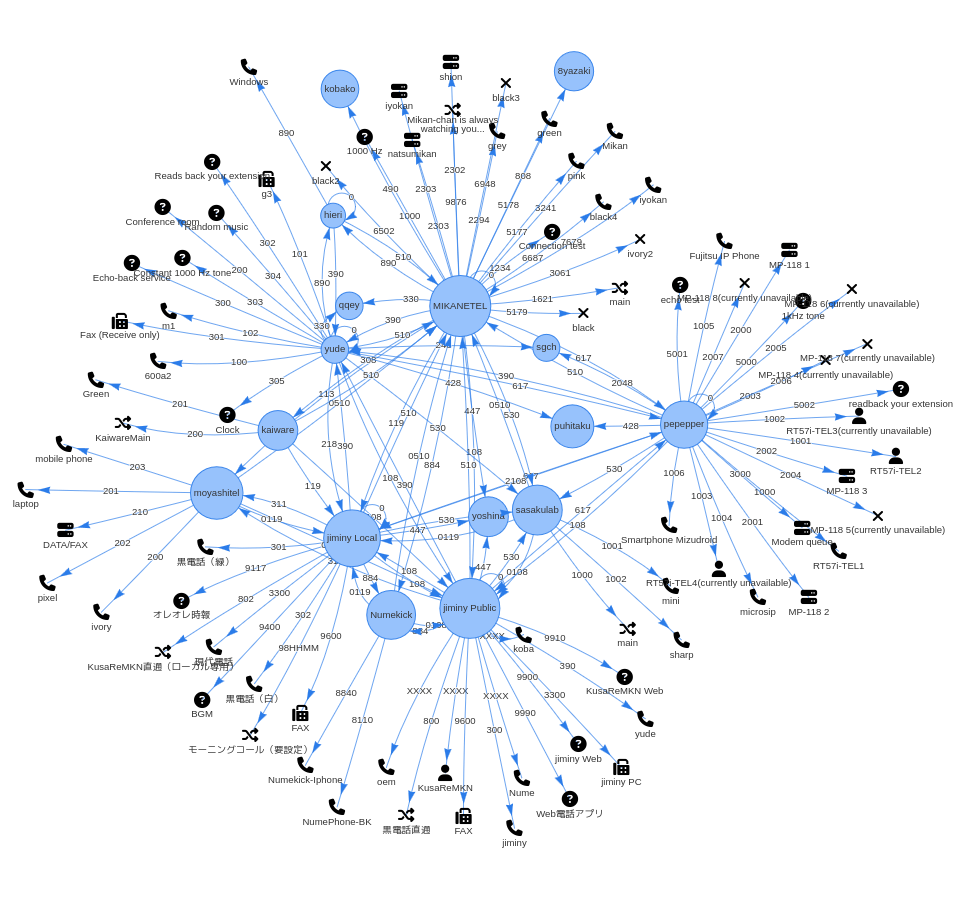
\includegraphics[height=\textheight]{./images/mantela.png}
    \end{column}
  \end{columns}
  \note{
    現在の電話網の姿を描画してみたよ。
    かなり小さくない網になっていることがわかると思うよ。

    この電話網の中には16個以上の電話局があって、
    端末数は68以上(隠されている端末もあるので実際には70数台)あるよ。
  }
\end{frame}

\begin{frame}
  \frametitle{現在の東京広域電話網の姿}

  \begin{columns}
    \begin{column}{.25\textwidth}
      \begin{description}[labelwidth=\linewidth]
        \item[交換局数]
          16局
        \item[端末数]
          68以上\\
          (仮想含む)
        \item[黒電話の数]
          15程度
        \item[その他]
          公衆電話\\
          ワープロ
      \end{description}
      ~
    \end{column}
    \begin{column}{.7\textwidth}
      \centering
      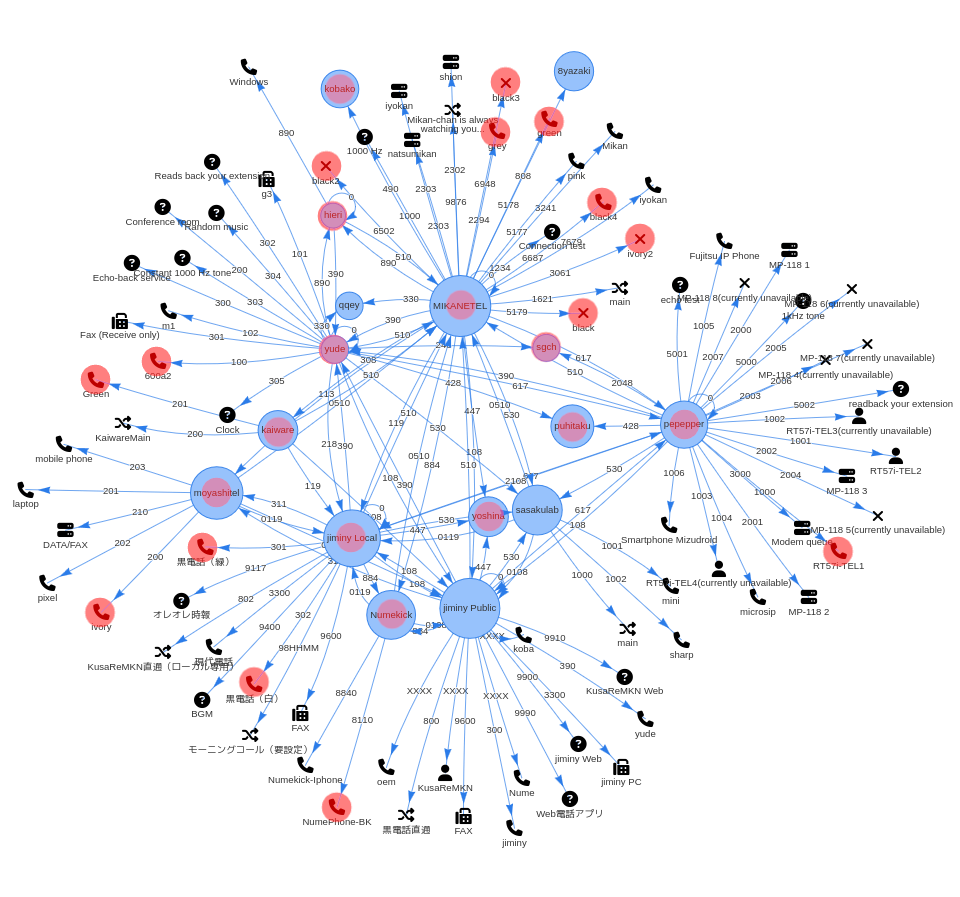
\includegraphics[height=\textheight]{./images/mantela2.png}
    \end{column}
  \end{columns}
  \note{
    もともと黒電話を使うことを念頭に作られた網であるので、
    黒電話を数えてみると15程度ありそうだよ。
    黒電話を収容している局は全16局中12局もあるよ(なんで?)。

    その他にも、公衆電話が接続されていたり、
    ワープロが接続されていたりとかなり面白い網になっているよ。
  }
\end{frame}

\section{みんなも「でんわ」をしよう!}
\note{
  さて、ここまでの話を聞いて
  みんなも「でんわ」をしたくなっている頃だと思うので
  巻き込み活動を開始していくよ。
}

\begin{frame}
  \frametitle{用意するもの}

  特にこだわらなければ必須なものは\textbf{コンピュータだけ}\\
  \hspace{1.5\zw}交換局を設置・相互接続するだけでOK(ソフト電話可)
  \\~\\[-.5\baselineskip]

  黒電話やFAXなど物理的な端末をぶら下げたい場合は……

  \begin{description}[labelwidth=\linewidth]
    \item[VoIPルータ(ゲートウェイ?)]
      IP通信を電話信号に変換する人\\
      YAMAHA RT57iやRT58iなどで動作確認済\\
      ICOM VE-TA10もインチキすれば動作可能
    \item[端末それ自体]
      電話線の刺さるものはだいたい友達
  \end{description}
  \note{
    交換局を電話網に接続するだけであれば、
    必要なものは交換局だけなので、
    適当なコンピュータがあれば始められるよ(x86\_64であればOK)。

    実際の端末、例えば黒電話やFAXなどを接続するにはもう数品必要だよ。
    VoIPルータと端末それ自体だよ。
    VoIPルータはYAMAHAのものが安定して稼動しているよ。
    これはヤフオクやメルカリでよく手に入るという報告を受けているよ。
    黒電話も同様だよ。
    みんなもしようね。
  }
\end{frame}

\begin{frame}
  \frametitle{今日のお話の記事(宣伝)}

  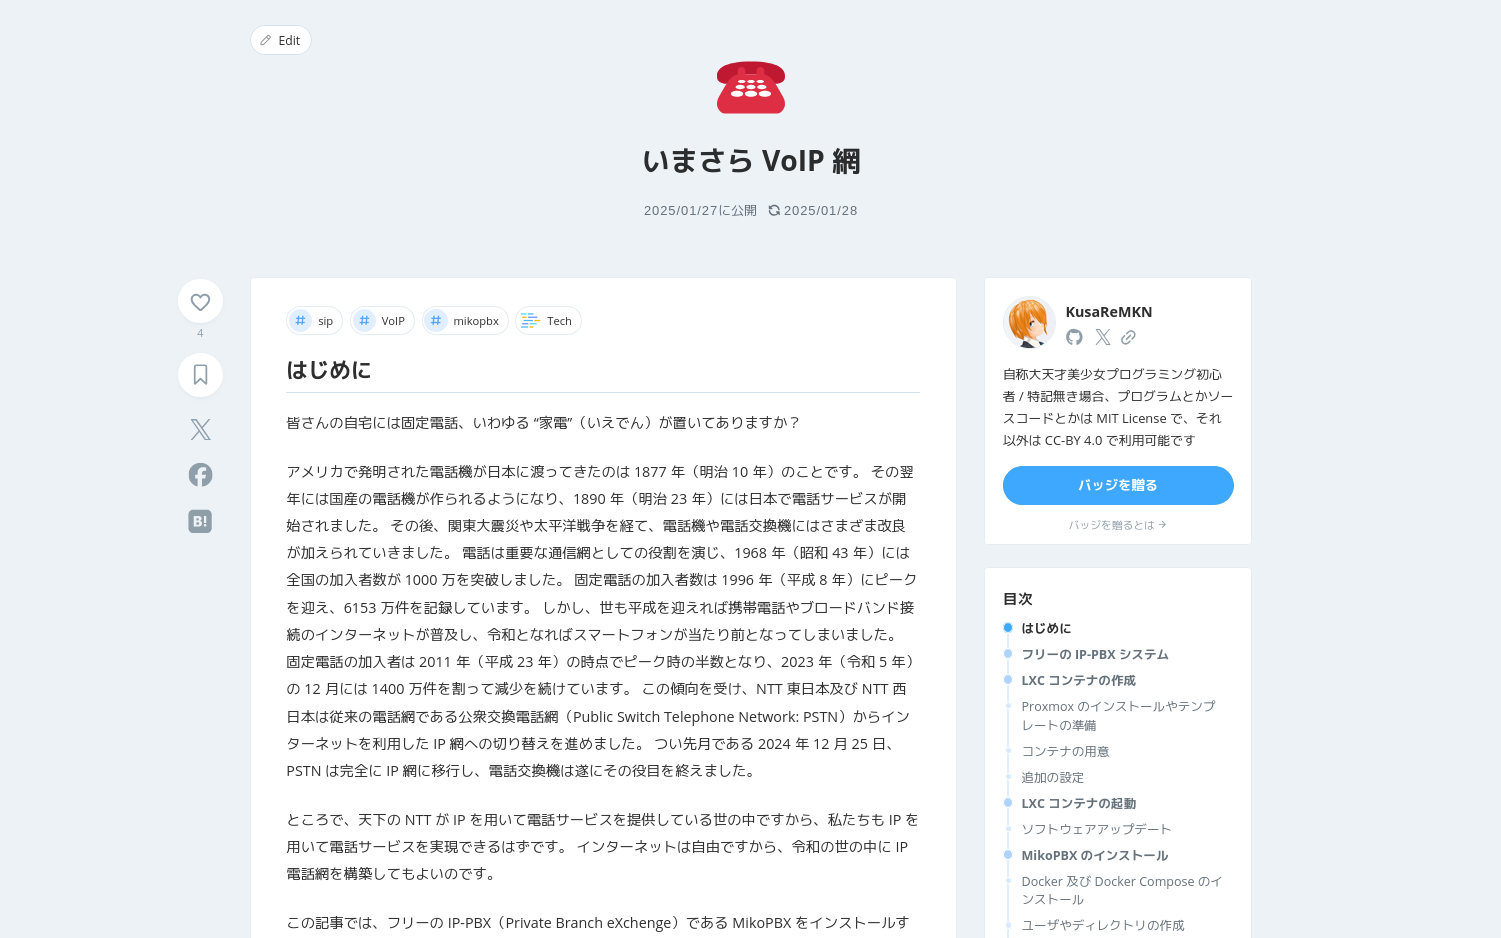
\includegraphics[width=\linewidth]{./images/imasara.png}
  \note{
    で、宣伝だよ。
    接続する方法の全てがZennに書いてあるよ。
  }
\end{frame}

\begin{frame}
  \frametitle{今日のお話の記事(宣伝)}

  \begin{description}[labelwidth=\linewidth,itemsep=\zh]
    \item[いまさらVoIP網]
      {\small
      \url{https://zenn.dev/kusaremkn/articles/abd760f9f2f450}}
    \item[VoIPルータを使って黒電話をIP電話機にする]
      {\small
      \url{https://zenn.dev/kusaremkn/articles/187222dc1d4f1d}}
    \item[ICOM VE-TA10を使うためにパケットを書き換えたりする]
      {\small
      \url{https://zenn.dev/kusaremkn/articles/cb32b500fc1334}}
  \end{description}
  \note{
    いまさらVoIP網でGoogleすると引っ掛かるハズなので、
    でんわをしてみたい人は検索してみてね。
  }
\end{frame}

\begin{frame}
  \frametitle{東京広域電話網コミュニティ}

  \begin{description}[labelwidth=\linewidth,itemsep=\zh]
    \item[Web site]
      {\small
      \url{https://tkytel.github.io/}}
    \item[Discord]
      {\small
      \url{https://discord.com/invite/QEzAnuSy9S}}
    \item[Mailing list]
      {\small
      \url{https://groups.google.com/g/tkytel}}
  \end{description}
  \note{
    東京広域電話網のコミュニティがあるよ。
    気軽に参加してみてね。
  }
\end{frame}

\section{まとめ}
\note{
  今日のおはなしのまとめだよ。
}

\begin{frame}
  \frametitle{オレオレIP電話網と黒電話で遊んでみた}

  IP-PBXシステムを利用したIP電話網を構築

  交換局同士の相互接続・多局接続を実現

  交換局ホップの実現(相互接続されていない局間での通話)

  \note{
    オレオレIP電話網と黒電話で遊んでみたことについてお話をしたよ。
    MikoPBXというIP-PBXを用いてIP電話網を構築してみたよ。
    交換局同士の相互接続を実現できたし、
    多局接続を実現できたので本当に網になったよ。
    交換局ホップを実現して、
    直接相互接続されていない局でも通話できることを確認したよ。
  }
\end{frame}

\begin{frame}[standout]
  おわりです
  \note{
    発表おわり〜
  }
\end{frame}

\end{document}
% ex: se et ts=2 :
